\section{Small and large polarons}
In the previous sections, we have divided polarons in two categories: small and large. A small polaron is defined as a polaron that is created by a distortion of the lattice smaller than the unit cell. Conversely, a large polaron originates from a distortion bigger than the unit cell. The distinction can also be made in terms of the strength of the electron-phonon coupling. When it is strong, electrons are localized around a single atom and only the interactions with the nearest-neighbors atoms are relevant. When the interaction is weak, longer-range interactions becomes more significant. A picture of the charge isosurfaces of a small and large polaron is given in \cref{fig:small_large}

We have seen how the two types of polarons are usually described with two different Hamiltonians. The Fröhlich Hamiltonian is typically used for large polarons, where the discreteness of the lattice plays a minor role. For this reason, large polarons are often also called Fröhlich polarons. On the other hand, small polarons - which are also called Holstein polarons - are described by the Holstein Hamiltonian, which takes into account the discrete behavior of the lattice more accurately.

The differences between small and large polarons are more than just their sizes. A very important one is their mobility \cite{natanzon2020}. Polarons form in polarizable materials, such ionic crystals or polar semiconductors. In both cases, electronic transport occur via hopping. The charges are thermally activated over a gap, and hop from one site to another. However, if in semiconductors the charges must have enough energy to jump over the band gap, in polaronic materials the gap is much narrower. In fact, polarons have to jump from a localized state (the polaronic band) to the conduction band.

Several different diffusion mechanisms have been identified to describe polarons mobility. However, a simplified picture can be drawn to highlight the general differences between small and large polarons \cite{franchini2021b}. Small polarons typically hop from one site to another assisted by phonons, when the distortion of the polaron's site is disturbed by thermal vibrations. The resulting motion is thus incoherent and the mobility is usually much smaller than \SI{1}{cm^2 V^{-1}s^{-1}}. The mobility increases with temperature, since this increases the thermal vibrations which cause the hoping. Conversely, large polarons tend to follow a quasi-free-carrier-like motion. We have seen that the effective mass is greater for polarons than for free-charge. Since the large effective mass prevents them from scattering with the phonon field, this results in a higher mobility. The mobility is reduced by the increasing of temperature, which makes the scattering more effective.

The property of small and large polarons discussed above are summarized in \cref{tab:small_large}.

\newcommand{\tabitem}{~~\llap{\textbullet}~~}
\begin{table}[p]
    \centering
    \caption{Summary of small and large polarons properties. The table is taken from Franchini's review on polarons \cite{franchini2021b}}.
    \label{tab:small_large}
    \begin{tabular}{ll}
        \toprule
        \multicolumn{1}{c}{
        Small (Holstein) polarons                  }        & \multicolumn{1}{c}{ Large (Fröhlich) polarons                 } \\
        \midrule
        \multicolumn{1}{c}{
        $\oper{H}_\text{el-ph} = \frac{g}{\sqrt{N}}\sum_{\vec{k}, \vec{q}} \adjop{c}_{\vec{k}+\vec{q}} \oper{c}_\vec{k} (\adjop{b}_{-\vec{q}} + \oper{b}_\vec{q})$
        }                                                   & \multicolumn{1}{c}{
        $\oper{H}_\text{el-ph} = \sum_{\vec{k}\vec{q}} M_{\vec{q}}\adjop{c}_{\vec{k}}\oper{c}_{\vec{k}-\vec{q}} (\oper{b}_{\vec{q}} + \adjop{b}_{-\vec{q}})$          }
        \\
        \midrule
        \tabitem Short-range electron-phonon interaction    & \tabitem Long-range electron-phonon interaction                 \\
        \tabitem Polaron radius $\approx$ lattice parameter & \tabitem Polaron radius $\gg$ lattice parameter                 \\
        \tabitem Narrow mid-gap electronic state            & \tabitem Shallow mid-gap electronic state                       \\
        $\qquad (\approx \SI{1}{eV}$ below $E_F$)           & $\qquad (\approx \SI{10}{eV}$ below $E_F$)                      \\

        \tabitem Incoherent motion (phonon assisted)        & \tabitem Coherent motion                                        \\
        \tabitem Thermally activated hopping mobility       & \tabitem Free carrier mobility                                  \\
        $\qquad \ll \SI{1}{cm^2 V^{-1} s^{-1}}$             & $\qquad \gg \SI{1}{cm^2 V^{-1} s^{-1}}$                         \\
        \tabitem Mobility increasing with temperature       & \tabitem Mobility decreasing with temperature                   \\
        \bottomrule
    \end{tabular}
\end{table}

\begin{figure}[p]
    \begin{subfigure}[b]{0.42\textwidth}
        \centering
        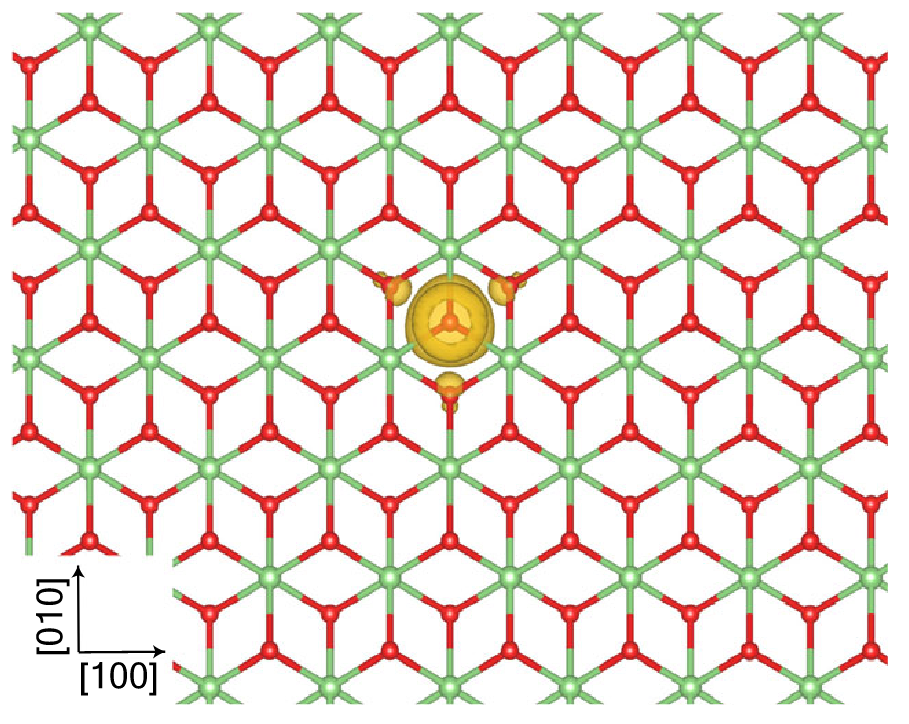
\includegraphics[width=\textwidth]{figures/small.png}
        \caption{Small polaron}
        \label{fig:small}
    \end{subfigure}
    \hfill
    \begin{subfigure}[b]{0.49\textwidth}
        \centering
        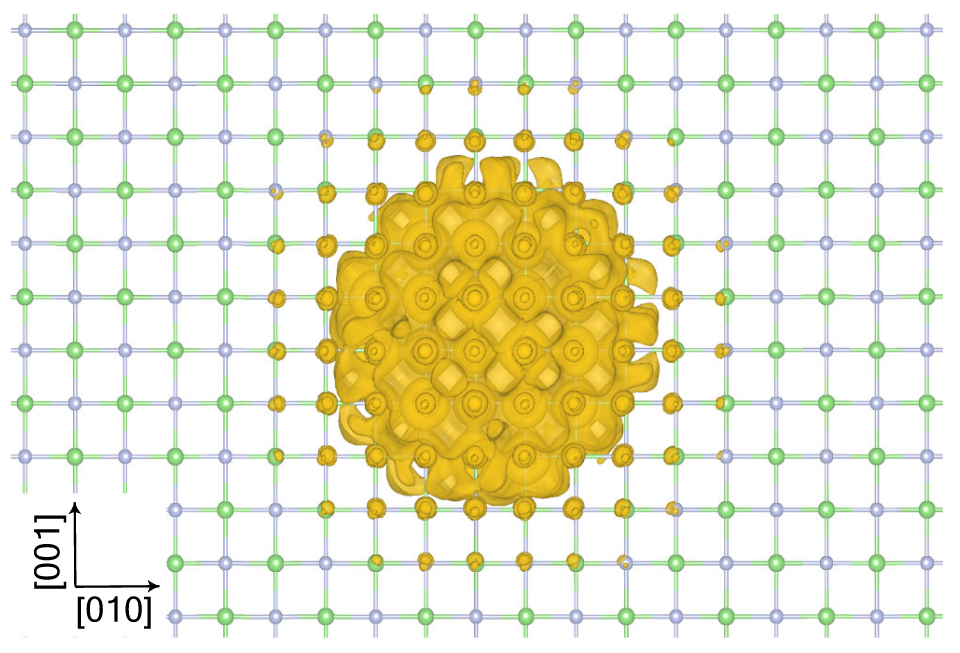
\includegraphics[width=\textwidth]{figures/large.png}
        \caption{Large polaron}
        \label{fig:large}
    \end{subfigure}
    \caption[Charge isosurfaces of a small and a large polaron]{Example of charge isosurfaces of a small and a large polaron in a 2D lattice. The images are taken from Sio et al. \cite{sio2019}}.
    \label{fig:small_large}
\end{figure}
\vfill